\documentclass[9.5pt, a4paper]{article}

\usepackage[utf8]{inputenc}
\usepackage[T1]{fontenc}
\usepackage[french]{babel}
\usepackage[margin=1cm, top=0.9cm, bottom=0.9cm]{geometry}
\usepackage{amsmath}
\usepackage{xcolor}
\usepackage{graphicx} % Ajout nécessaire pour afficher les images avec \includegraphics
\usepackage{hyperref}
\usepackage{enumitem}
\usepackage{titlesec}
\usepackage{tikz}
\usepackage[absolute,overlay]{textpos}

\setlength{\parindent}{0pt}
\setlist{topsep=1pt, itemsep=0pt, parsep=0pt}

% Définition de la couleur bleu moderne (style image 2)
\definecolor{cvblue}{RGB}{51, 102, 204}

\hypersetup{
    colorlinks=true,
    linkcolor=cvblue,
    urlcolor=cvblue
}

% Format des sections (titre en bleu avec une ligne horizontale sous le titre)
\titleformat{\section}
  {\large\bfseries\color{cvblue}}
  {}{0em}{}
  [\color{cvblue}\titlerule]

\titlespacing*{\section}{0pt}{6pt}{2pt}

\pagestyle{empty}

\begin{document}

%----------------------------------------------------------------------------------------
%	EN-TÊTE / COORDONNÉES
%----------------------------------------------------------------------------------------
\noindent
\begin{minipage}[c]{2.4cm}
    \begin{tikzpicture}
        \node[circle, draw=cvblue, linewidth=1pt, minimum size=2.3cm, path picture={
            \node at (path picture bounding box.center){
                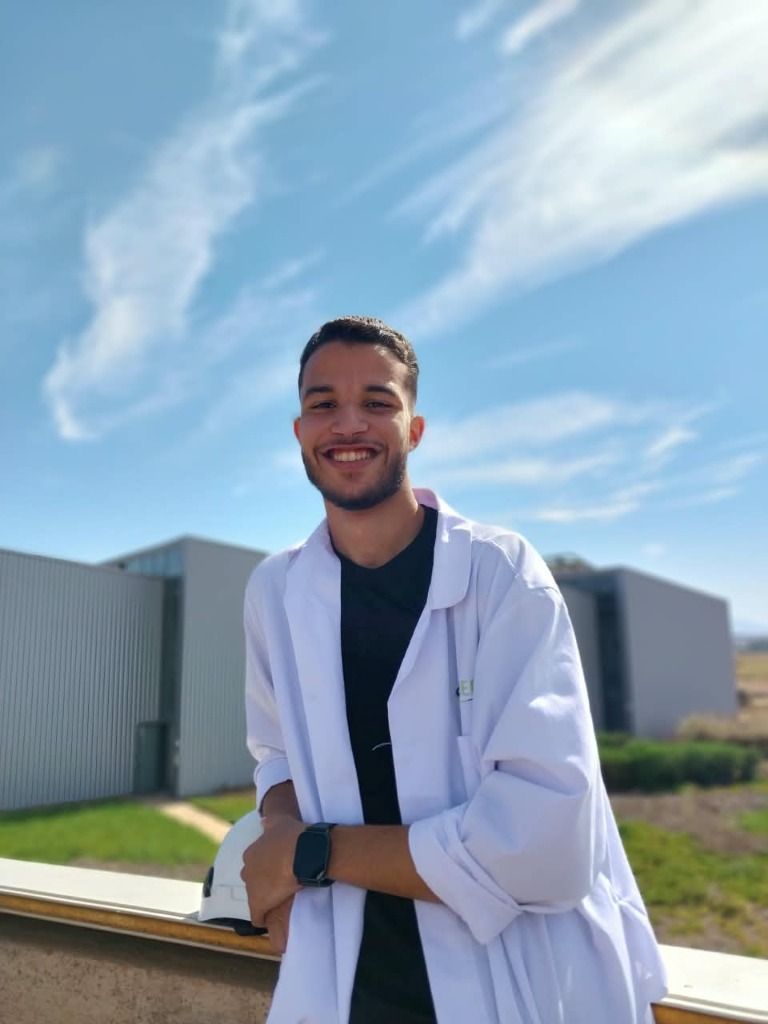
\includegraphics[width=2.6cm]{cremti.jpeg}
            };
        }] {};
    \end{tikzpicture}
    % Option sans TikZ si besoin :
    % 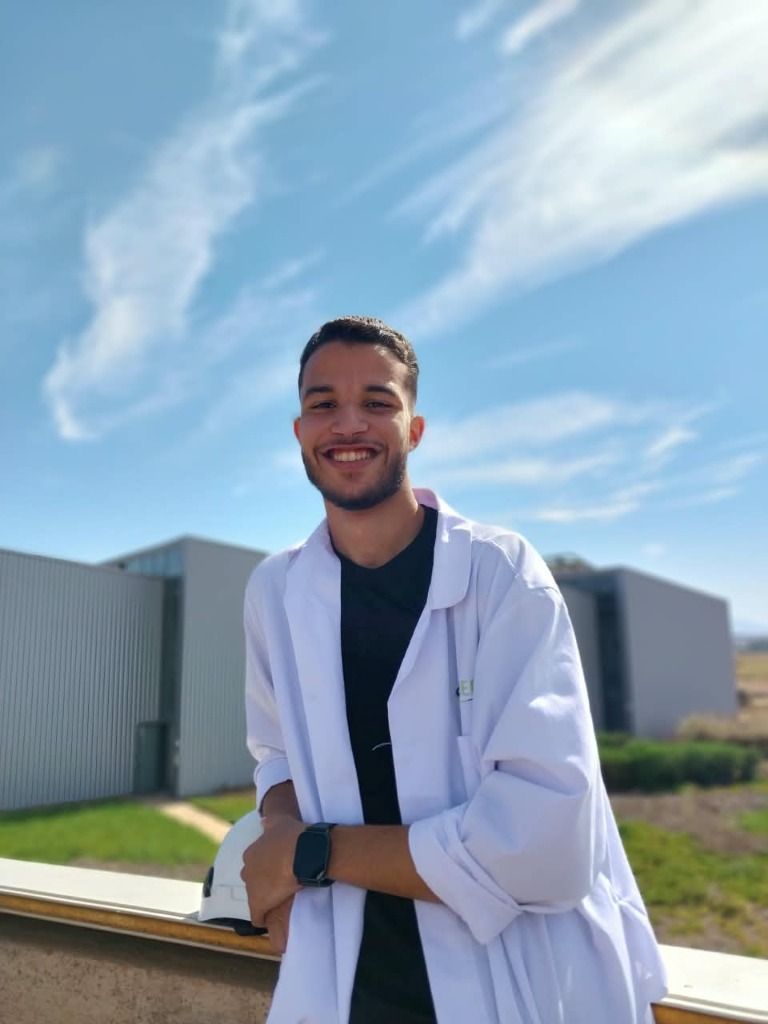
\includegraphics[width=2.3cm]{cremti.jpeg}
\end{minipage}%
\begin{minipage}[c]{15.9cm}
    \begin{center}
        {\Huge \textbf{Mohamed MEREHOUM}}\\[0.15em]
        {\large \textit{\color{cvblue}Technicien Spécialisé en Systèmes Énergie Solaire}}\\[0.3em]
        \href{mailto:mohamedmerehoum860@gmail.com}{mohamedmerehoum860@gmail.com}  \textbar{}  
        0672-992948  \textbar{}  
        Oujda, Maroc  \textbar{}  
        Permis B  \textbar{}  
        Mobilité Nationale
    \end{center}
\end{minipage}

\vspace{0.6em}

%----------------------------------------------------------------------------------------
%	PROFIL
%----------------------------------------------------------------------------------------
\section{Profil}
Passionné par les énergies renouvelables, je m'apprête à obtenir mon diplôme de Technicien Spécialisé en Systèmes Énergie Solaire à l'IFMEREE d'Oujda. Mon stage d'initiation m'a permis d'acquérir une première expérience concrète en installation et maintenance de systèmes solaires. Je suis actuellement à la recherche d'un stage de PFE afin de mettre en œuvre mes compétences et de participer à des projets innovants dans le domaine des énergies renouvelables.

%----------------------------------------------------------------------------------------
%	FORMATIONS
%----------------------------------------------------------------------------------------
\section{Formations}
\noindent
\textbf{IFMEREE, Oujda} --- \textit{Diplôme de Technicien Spécialisé en Énergies Renouvelables \& Équipements Solaire} \hfill 2024 -- 2026\\
\textbf{Lycée Elarbi Al Houcini, Oujda} --- \textit{Baccalauréat Sciences Physiques et Chimie} \hfill 2020 -- 2023

%----------------------------------------------------------------------------------------
%	EXPÉRIENCES PROFESSIONNELLES
%----------------------------------------------------------------------------------------
\section{Expériences Professionnelles}

\noindent
\textbf{Energy Pro Tech --- Oujda, Maroc} --- \textit{Stage PFE} \hfill Mars 2026 -- Juin 2026
\begin{itemize}[leftmargin=1.5em, label=---, itemsep=1pt, topsep=1pt]
    \item Réalisation des structures avec Fer H ou Profil C.
    \item Installation des panneaux photovoltaïques.
    \item Tirage des câbles DC et AC.
\end{itemize}

\vspace{0.1em}
\noindent
\textbf{Ecowatt --- Oujda, Maroc} --- \textit{Stage d'initiation} \hfill Juillet 2025 -- Août 2025
\begin{itemize}[leftmargin=1.5em, label=---, itemsep=1pt, topsep=1pt]
    \item Gestion des relations avec les clients et élaboration des propositions commerciales.
    \item Participation aux visites de chantier.
\end{itemize}

\vspace{0.1em}
\noindent
\textbf{IFMEREE --- Oujda, Maroc} --- \textit{Étudiant en Systèmes Énergie Solaire} \hfill 2024 -- 2026
\begin{itemize}[leftmargin=1.5em, label=---, itemsep=1pt, topsep=1pt]
    \item Apprentissage des techniques de la mise en service des installations.
    \item Câblage des coffrets DC et AC, maîtrise des techniques de dimensionnement.
\end{itemize}

%----------------------------------------------------------------------------------------
%	PROJETS ACADÉMIQUES
%----------------------------------------------------------------------------------------
\section{Projets Académiques}
\begin{itemize}[leftmargin=1.5em, label=---, itemsep=1pt, topsep=1pt]
    \item \textbf{Projet d'installation solaire photovoltaïque à LEAR Meknès (1,4 MW) :} Installation des panneaux photovoltaïques EST-OUEST. Préparation du rapport PVSol, modélisation 3D sur SketchUp, et planification du projet via Gantt.
    \item \textbf{Projet d'installation solaire photovoltaïque à Heirchmane Kénitra (711 kW) :} Élaboration des notes de calculs sur Excel, préparation du rapport PVsyst incluant les émissions de $\text{CO}_2$, et rédaction du rapport général sur Word.
    \item \textbf{Projet d'installation des panneaux photovoltaïques dans la toiture de la salle B à IFMEREE Oujda (170,5 $\text{m}^2$) :} Visite du local pour prendre les mesures, élaboration des plans et schémas sur AutoCAD, et dimensionnement de l'installation sur PVsyst.
\end{itemize}

%----------------------------------------------------------------------------------------
%	COMPÉTENCES TECHNIQUES & INFORMATIQUE
%----------------------------------------------------------------------------------------
\section{Compétences Techniques}
\begin{itemize}[leftmargin=1.5em, label=---, itemsep=1pt, topsep=1pt]
    \item \textbf{Projection des plans 2D en 3D sur SketchUp :} Conversion des plans 2D en 3D en projetant les plans AutoCAD avec leurs mesures sur SketchUp.
    \item \textbf{Dimensionnement des installations solaire thermique et photovoltaïque :} Élaboration des notes de calculs dans Excel, dimensionnement et choix du matériel sur PVsyst.
    \item \textbf{La mise en service des installations :} Vérification de passage du courant dans les câbles et programmation de l'onduleur.
    \item \textbf{Élaboration des schémas et plans électriques 2D sur AutoCAD :} Réalisation des schémas unifilaire et multifilaire, plans d'implantation, de câblage et de la mise à la terre des installations.
    \item \textbf{Maintenance des équipements et installations solaire thermique :} Maîtrise de la maintenance préventive et corrective, utilisation des appareils de mesure.
    \item \textbf{Câblage des coffrets DC et AC :} Maîtrise de dénudage et de sertissage des câbles.
    \item \textbf{Logiciels \& Outils :} Gantt Projects (cadre temporel et main d'œuvre), SketchUp, AutoCAD, PVsyst, Pack Office.
\end{itemize}

%----------------------------------------------------------------------------------------
%	LANGUES
%----------------------------------------------------------------------------------------
\section{Langues}
\begin{itemize}[leftmargin=1.5em, label=---, itemsep=1pt, topsep=1pt]
    \item \textbf{Arabe :} Langue maternelle
    \item \textbf{Français :} Courant
    \item \textbf{Anglais :} Technique
\end{itemize

%----------------------------------------------------------------------------------------
%	ATOUTS
%----------------------------------------------------------------------------------------
\section{Atouts \& Centres d'Intérêt}
\noindent
\textbf{Atouts :} Communication claire et écoute active, esprit analytique et résolution de problèmes, rigueur et sens du détail.

\end{document}
